\chapter{MINLP}
\newcommand{\lift}{\mathrm{lift}}
\newcommand{\ub}{\mathrm{ubbest}}
\newcommand{\F}{{\mathcal F}}

\subsection{Relaxations and Convex Hulls}

For a problem with a linear objective function

\begin{align}
\min c^\top x\\
 x\in \mathcal X
\end{align}
for some feasible set $\mathcal X$.  Let $p^*_{\mathcal X}$ denote the optimal objective value.
\begin{theorem}
Let $\mathcal F \subseteq \R^n$ (not necessarily convex) be compact and let $\mathcal R \supseteq \conv(\mathcal F)$.  Then 
$$
p^*_\mathcal F = p^*_{\conv(\mathcal{F})} \geq p^*_{\mathcal R},
$$
that is, 
\begin{enumerate}
\item optimizing over the convex hull of feasible solutions returns the same objective value,
\item optimizing over a relaxation returns a lower bound.
\end{enumerate}
\end{theorem}

\section{Extended Space and Spatial Branch and Bound}
We will discuss spatial branch and bound in the context of liftings of nonconvex problems to an extended space.  This means that we will reformulate the problem by adding new variables.  Specifically,  consider a quadratic optimization problem with linear constraints (where $Q$ is symmetric)

\begin{align}
\min\quad  &x^\top Q x + c^\top x\\
&Ax \leq b\\
&x \in \R^n
\end{align}

Let $\F = \{  x\in \R^n : Ax \leq b\}$ be the feasible region of the problem.

\subsubsection{Extended Space}

For any product terms $x_ix_j$ in the formulation, construct a new variable $Y_{ij}$ as
\begin{equation}
Y_{ij} = x_ix_j.
\end{equation}
If all product terms are present, this can be written as
\begin{equation}
Y = x x^\top.
\end{equation}
We will use this notation, although it is not always necessary to constructed a lifted variable when the corresponding products are not present.

Now the reformulation of the quadratic minimization problem can be written as 
\begin{align}
\label{lifted-problem}
\min\quad  &\tilde Q \circ Y + c^\top x\\
&Ax \leq b\\
& Y = x x^\top\\
&x \in \R^n\\
& Y \in \R^{n \times n}
\end{align}
The objective function is now linear, which is very nice!


Now, let
$$
\mathcal F_\lift = \{ (x,Y) \in \R^n \times \R^{n \times n}: Ax \leq b, Y = x x^\top\}.
$$

The set $\mathcal F$ is non-convex, which is hard to deal with.  So instead, we consider some convex relaxation $\mathcal R$ of $\conv(\mathcal F)$.  We restrict that 
$$
\conv(\mathcal F) \subseteq \mathcal R \subseteq \{ (x,Y) : Ax \leq b \},
$$
that is, we enforce the original constraints from $\F$ on the $x$ variables.  Thus, for any solution $(\bar x,\bar Y) \in \R$, although it may be that $(\bar x, \bar Y) \notin \mathcal F$, we do still have that $\bar x$ is feasible for the original problem.
\begin{align}
\label{relaxed-lifted-problem}
\min\quad  &\tilde Q \circ Y + c^\top x\\
&Ax \leq b\\
& (x,Y) \in \mathcal R
\end{align}

\subsection{Spatial Branch and Bound}
The goal of spatial branch and bound is to sequentially identify subregions of the feasible set with lower bounds that are worse than the best known feasible solution, and hence you can \emph{prune} (remove) that region from the space of 
places to look for an optimal solution.


In this algorithm, we build a \emph{branch and bound tree} that starts with a root node and then branches on nodes as we go.  

\begin{general}{Process at a node}{}
\textbf{Input:} A feasible region $\mathcal F^i \subseteq \F$, a upper bound $\ub$ on $p^*_{\F}$\\
\begin{enumerate}
\item Write down the lifted problem \eqref{lifted-problem}.
\item Construct a relaxation $\mathcal R$ of $\F_\lift^i$.
\item Optimize the relaxed lifted problem \eqref{relaxed-lifted-problem} and return an objective value $z^i$ and a point $(x^i,Y^i) \in \mathcal R$.   Note that 
\begin{itemize}
\item $x^i \in \F^i \subseteq \F$
\item $p^*_\F \leq p^*_{\F^i} \leq f(x^i)$
\item $p^*_{\F^i} \geq z^i$
\end{itemize}
\item If $f(x^i) < \ub$, set $\ub \leftarrow f(x^i)$.
\begin{enumerate}
\item If $\F^i = \emptyset$, i.e., is infeasible,  \textbf{prune this node.}
\item If $z^i > \ub$, \textbf{prune this node.}  No optimal solution for $\F$ can be found in $\F^i$.
\item If $f(x^i) = z^i$, then $p^*_{\F_i} = f(x^i)$.  Return $x^i$ and \textbf{prune this node: found an optimal solution in $\F^i$} (but this may not be optimal for $\F$).  
\item Else, if $z^i < f(x^i)$ and $z_i < \ub$, then \textbf{Branch!}.  Create two subproblems $\F^{i+1}$ and $\F^{i+2}$ such that $\F^i = \F^{i+1} \cup \F^{i+2}$, and process each node using this algorithm.
\end{enumerate}
\end{enumerate}


\end{general}
Here is an example of a branch and bound tree.  It is important that each node ends in either infeasible, suboptimal, or optimal for the subproblem $\F^i$.  Subproblems are created by changing lower or upper bounds on the variables $x_i$.   The numbers in the example are fictitious and do not come from any particular function.

\begin{center}
Step 0:
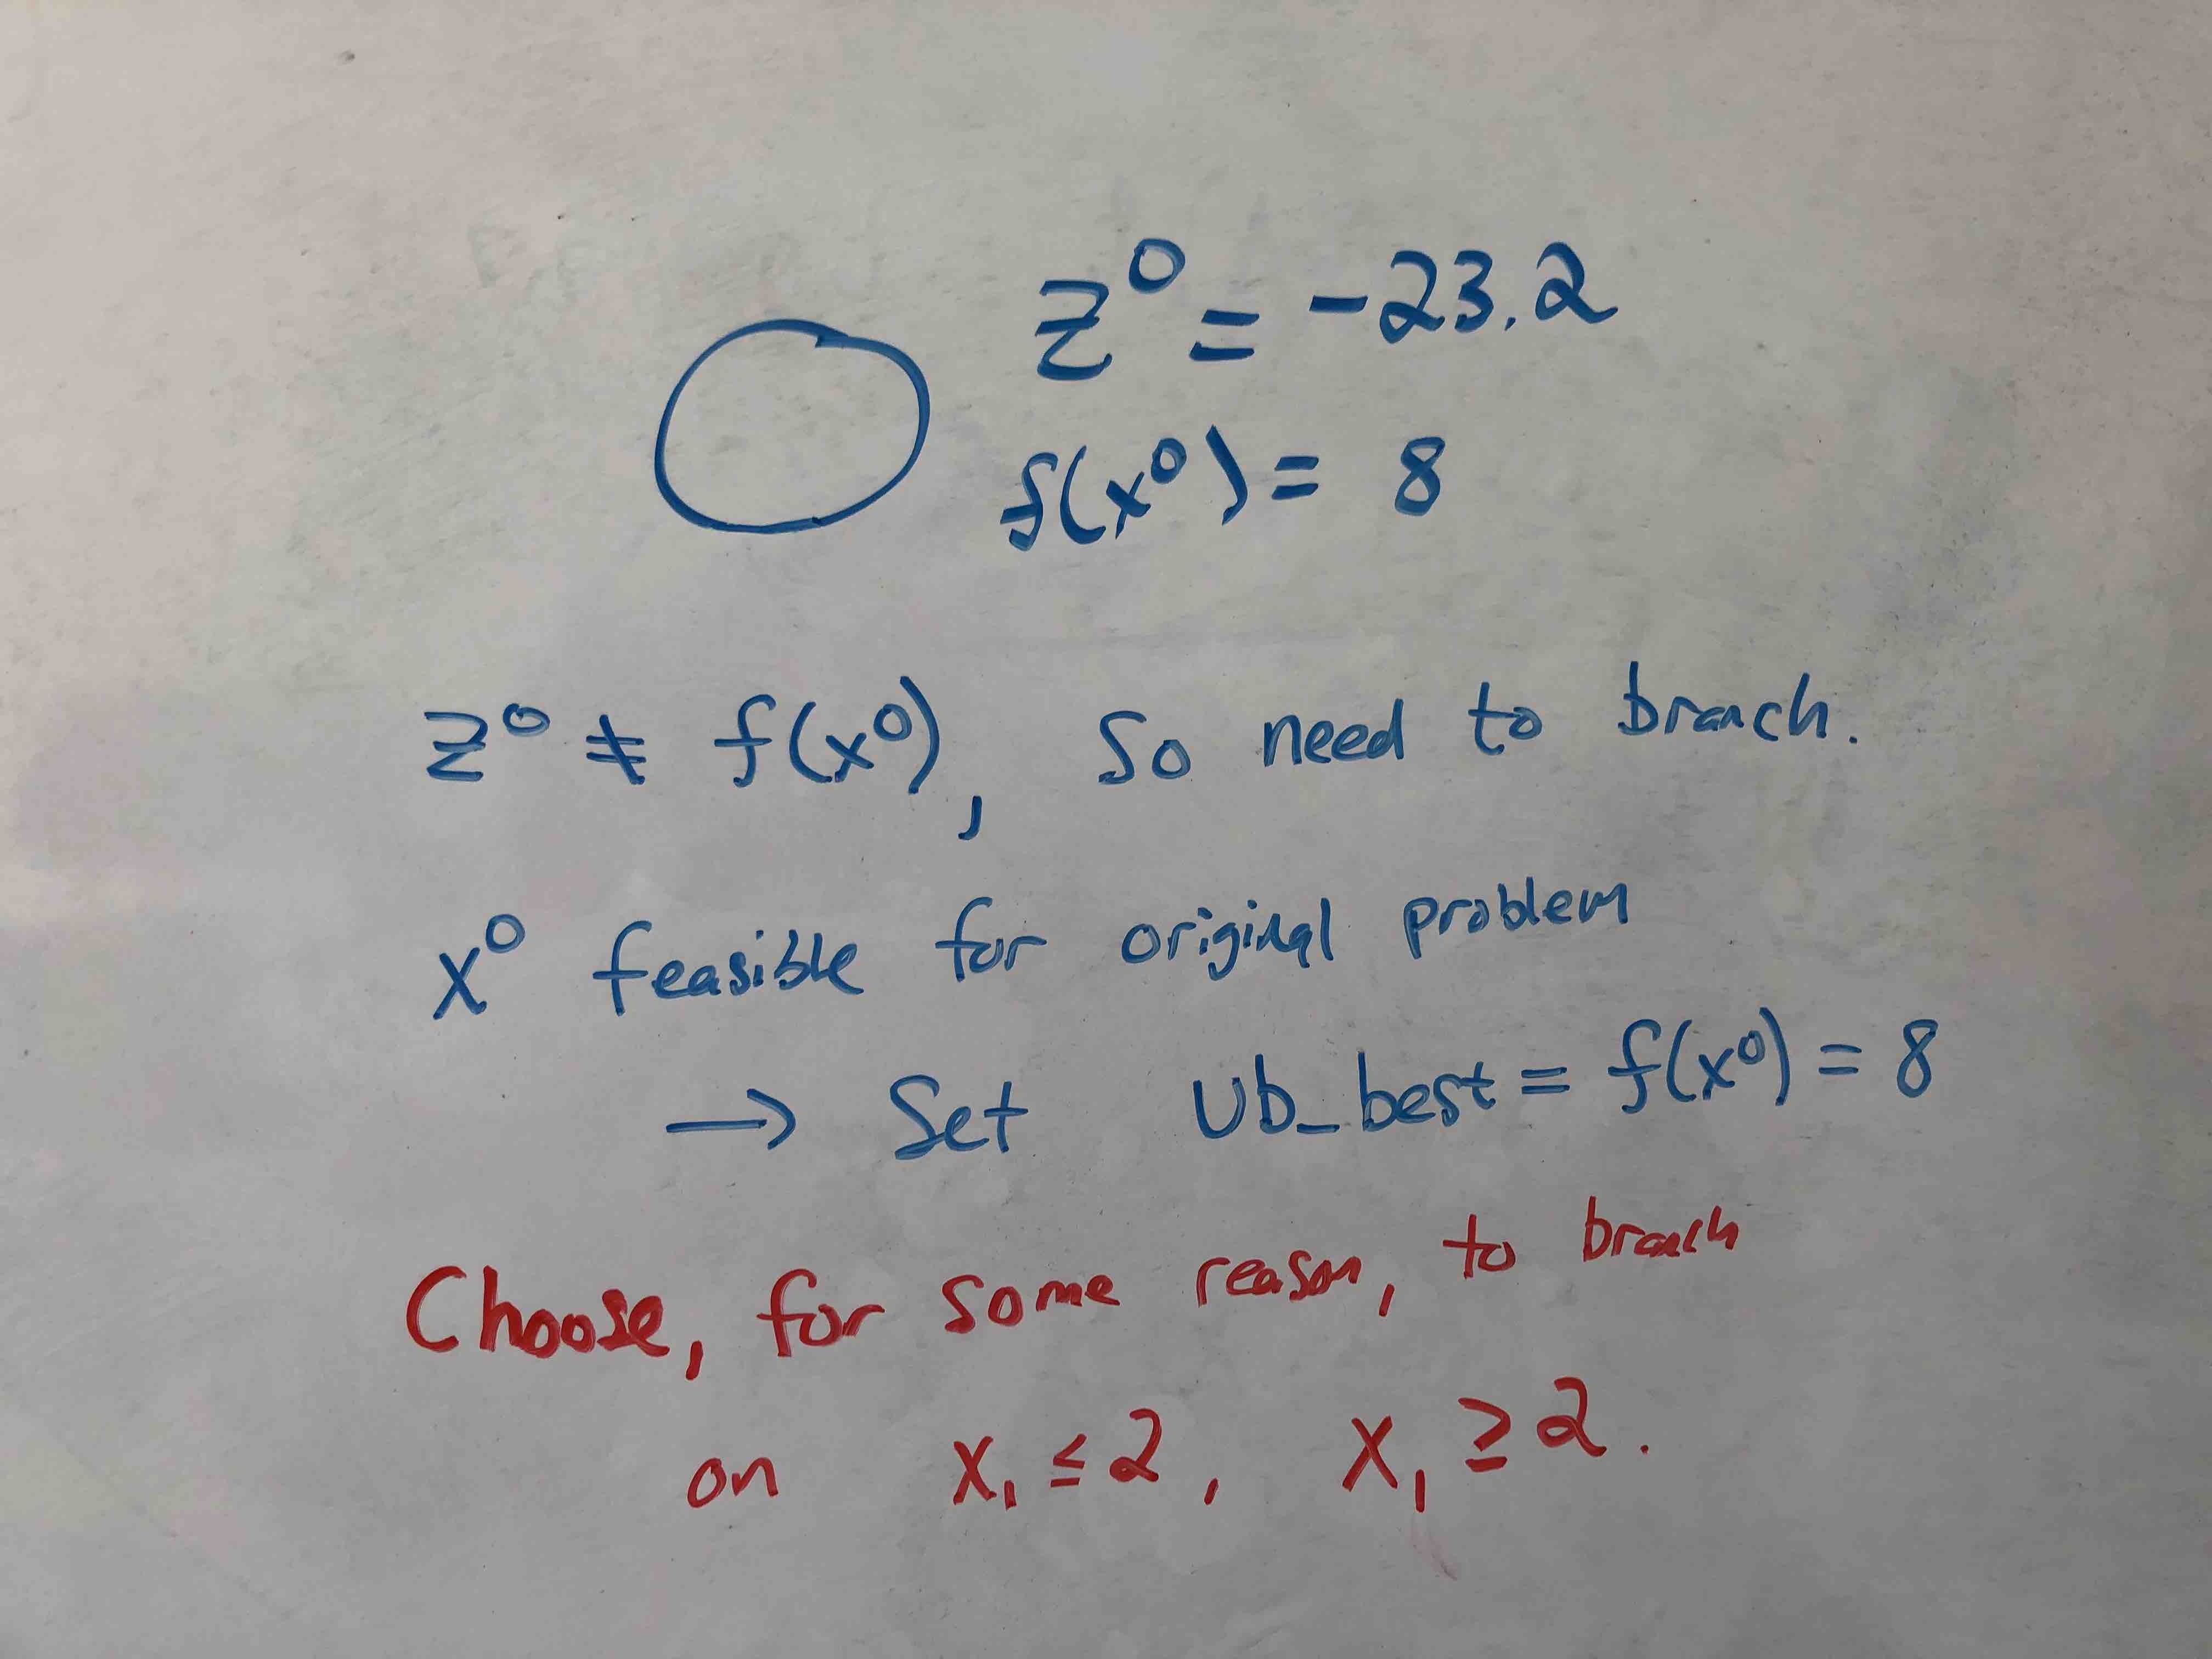
\includegraphics[scale = 0.06]{spatial_bnb_1}

Step 1:
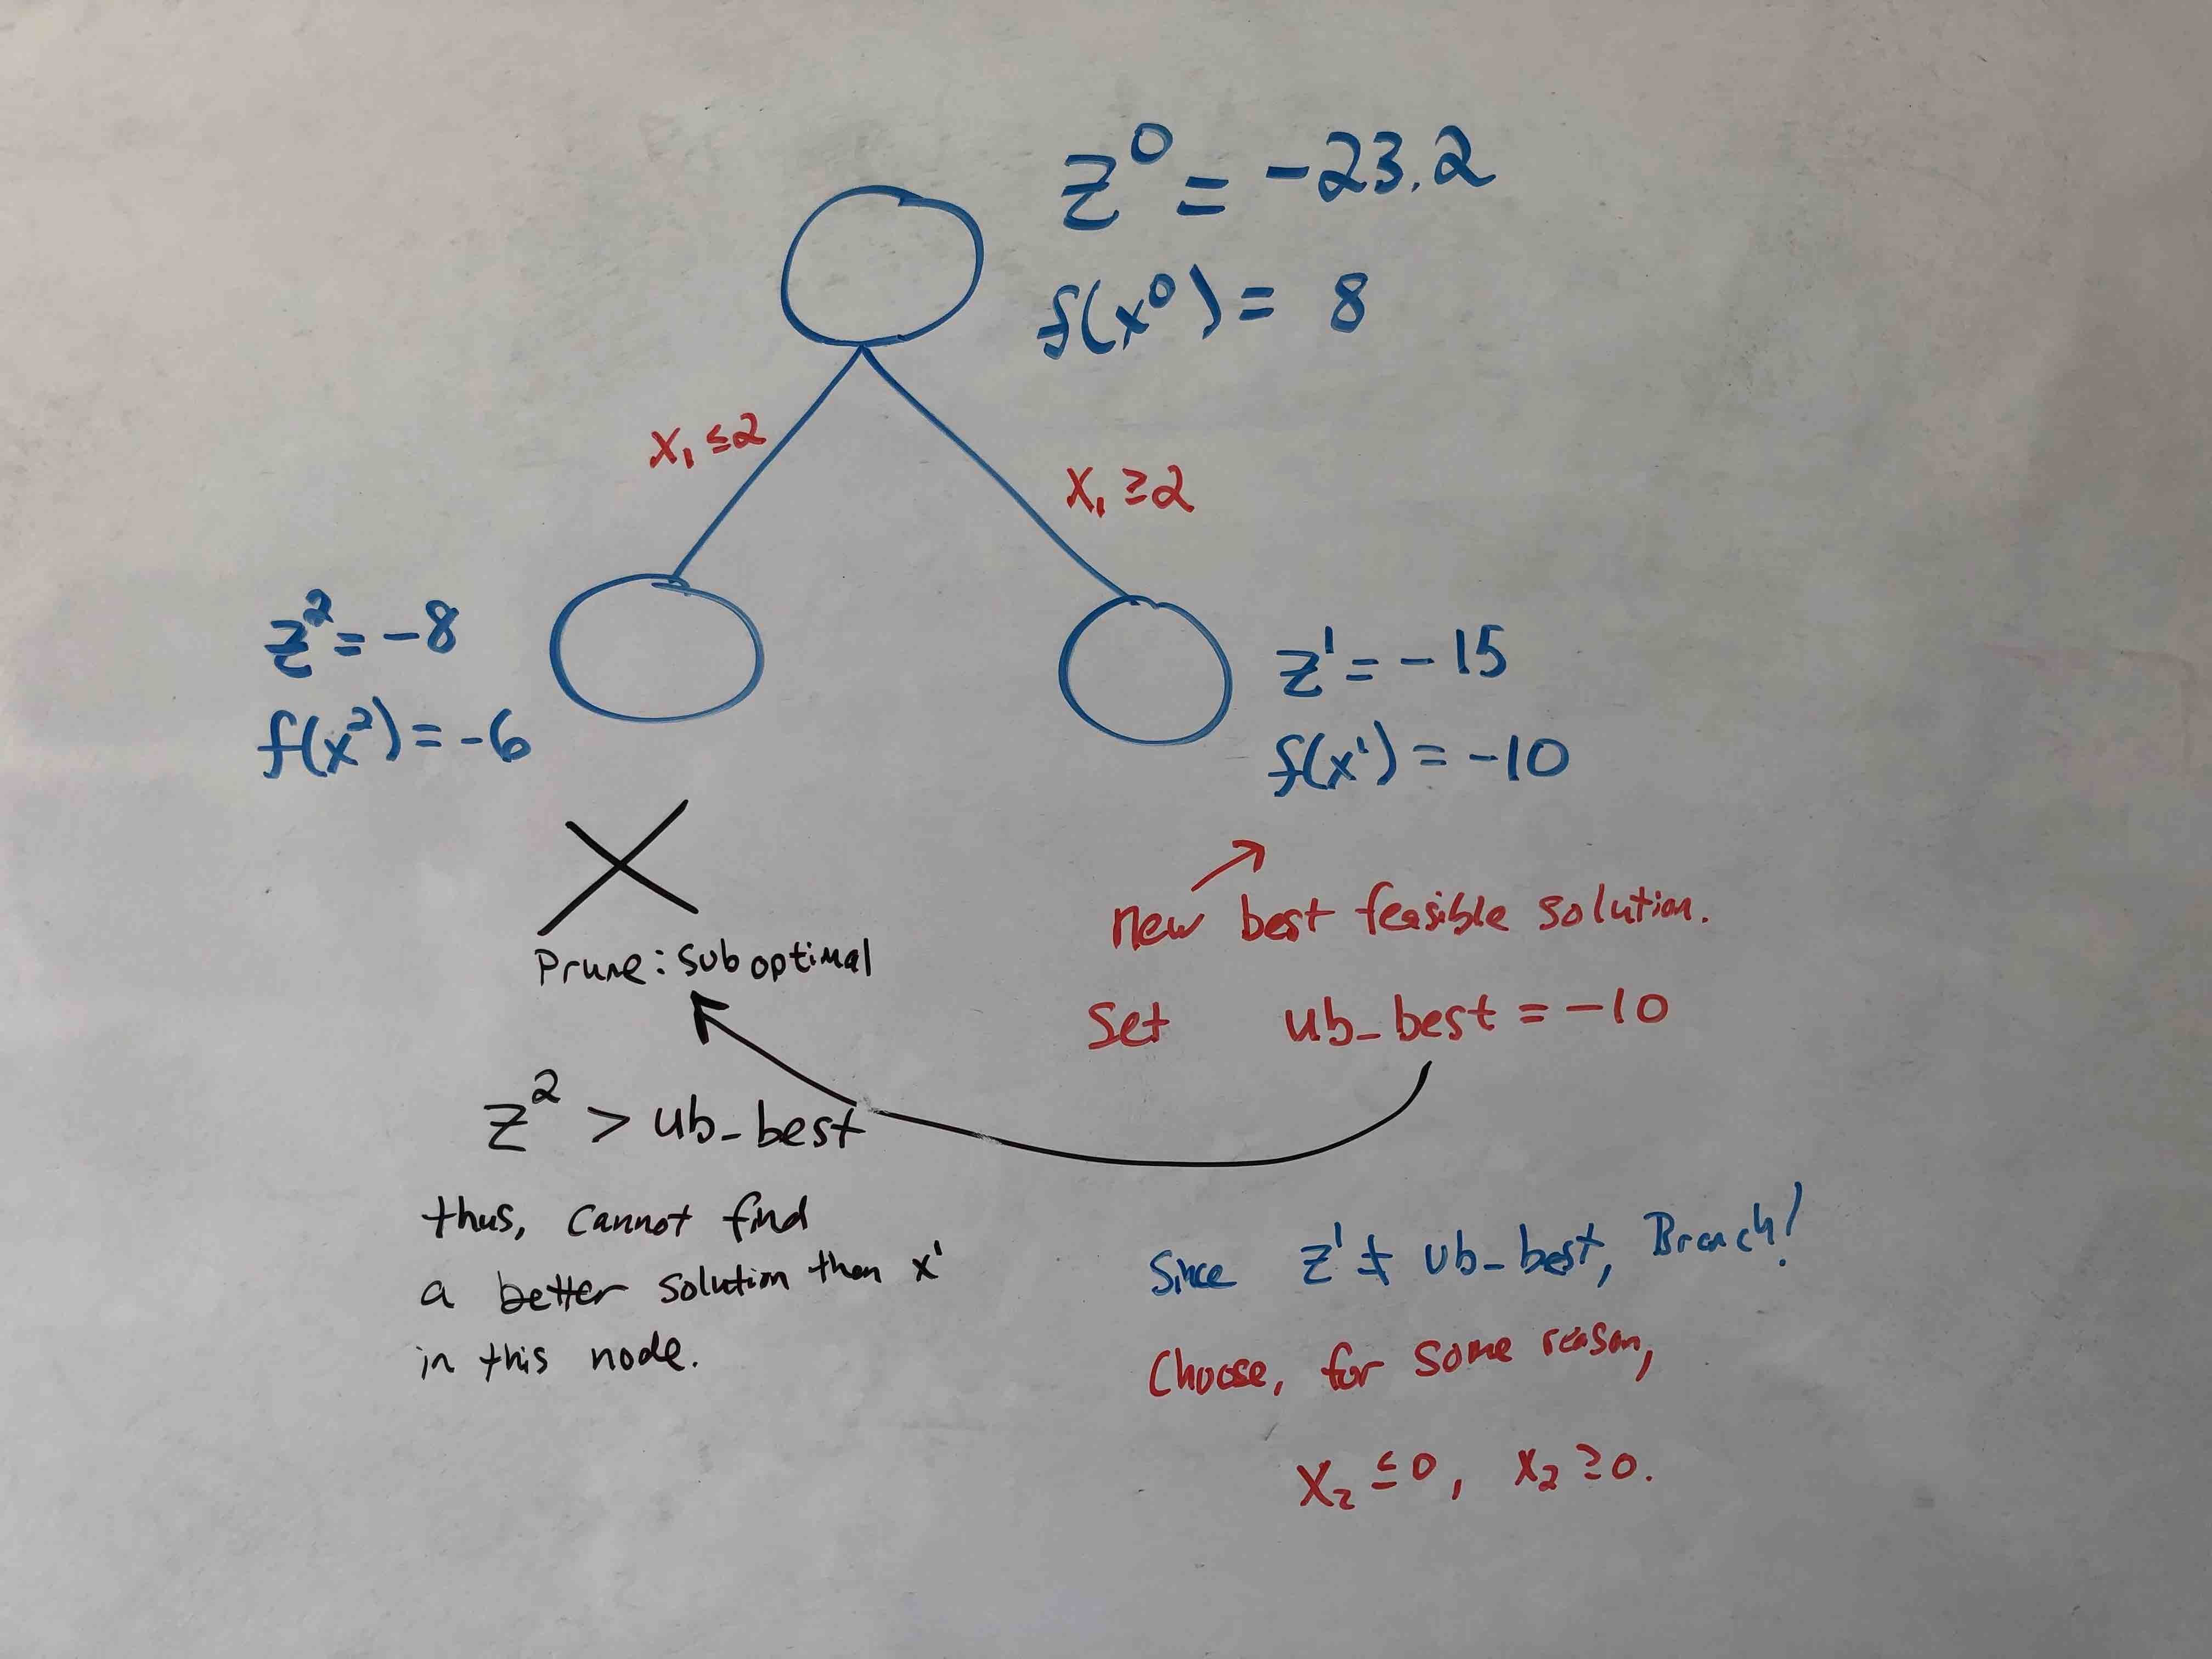
\includegraphics[scale = 0.08]{spatial_bnb_2}

Step 2:
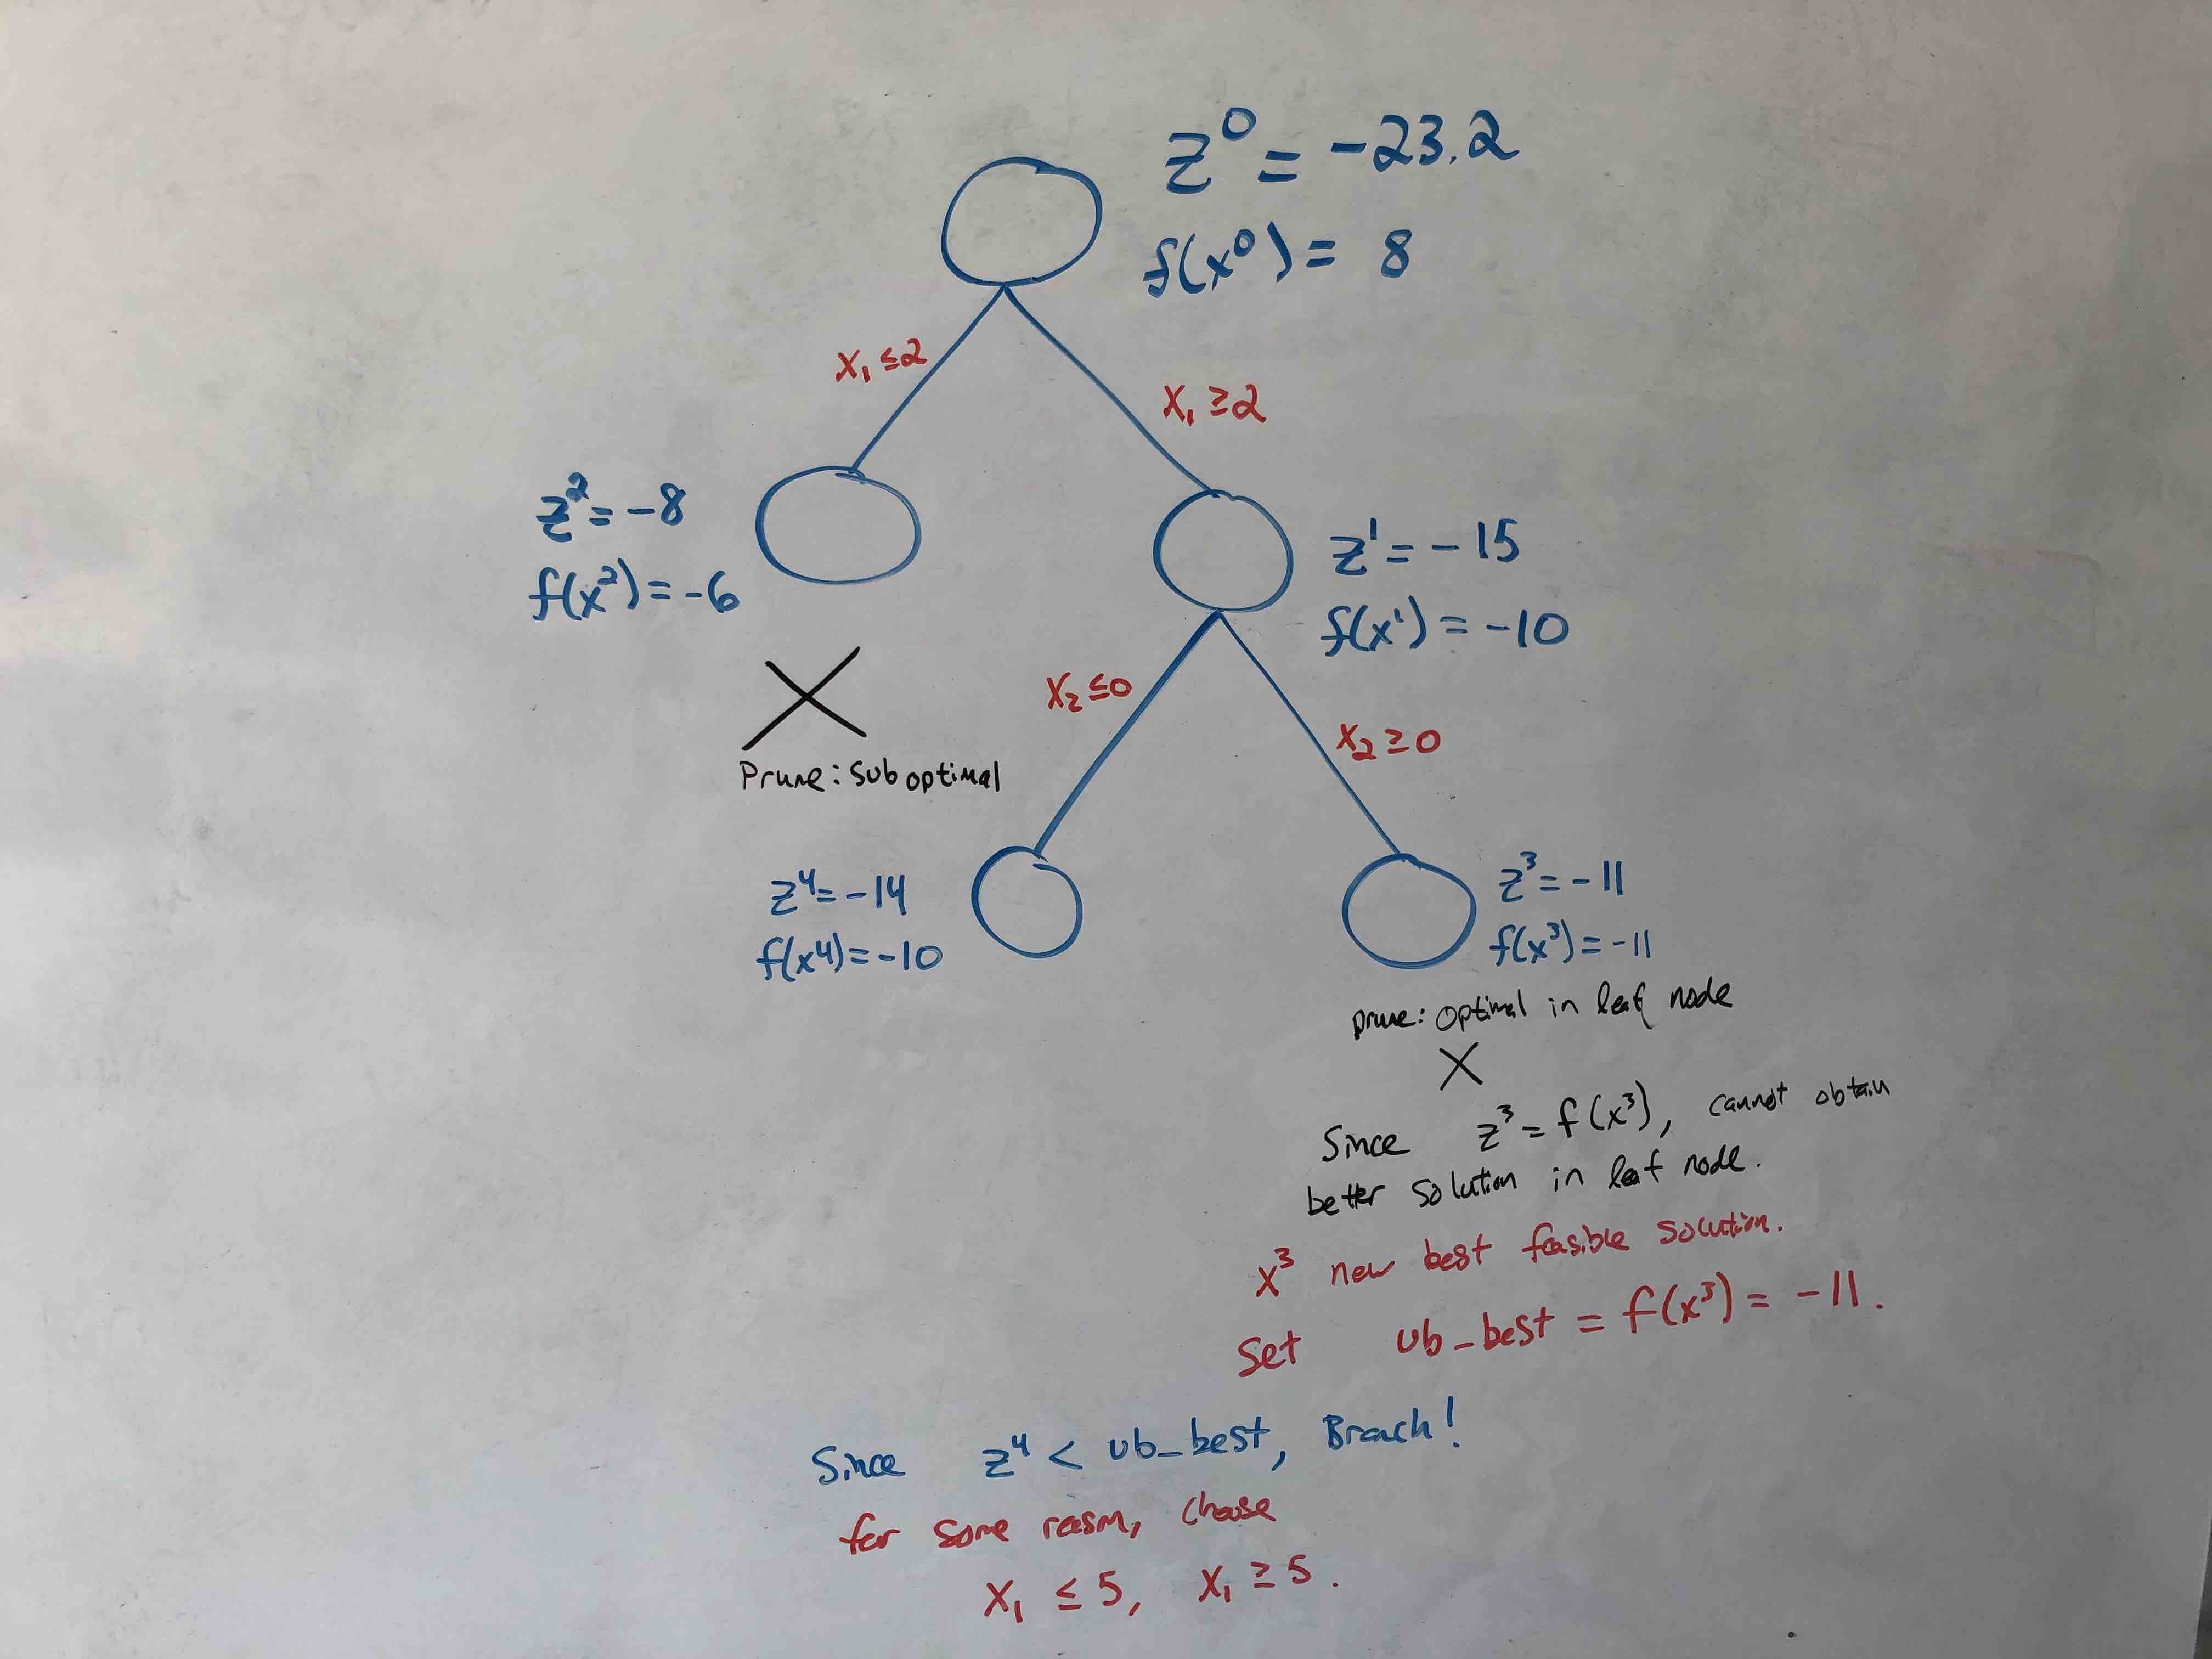
\includegraphics[scale = 0.09]{spatial_bnb_3}

Step 3:
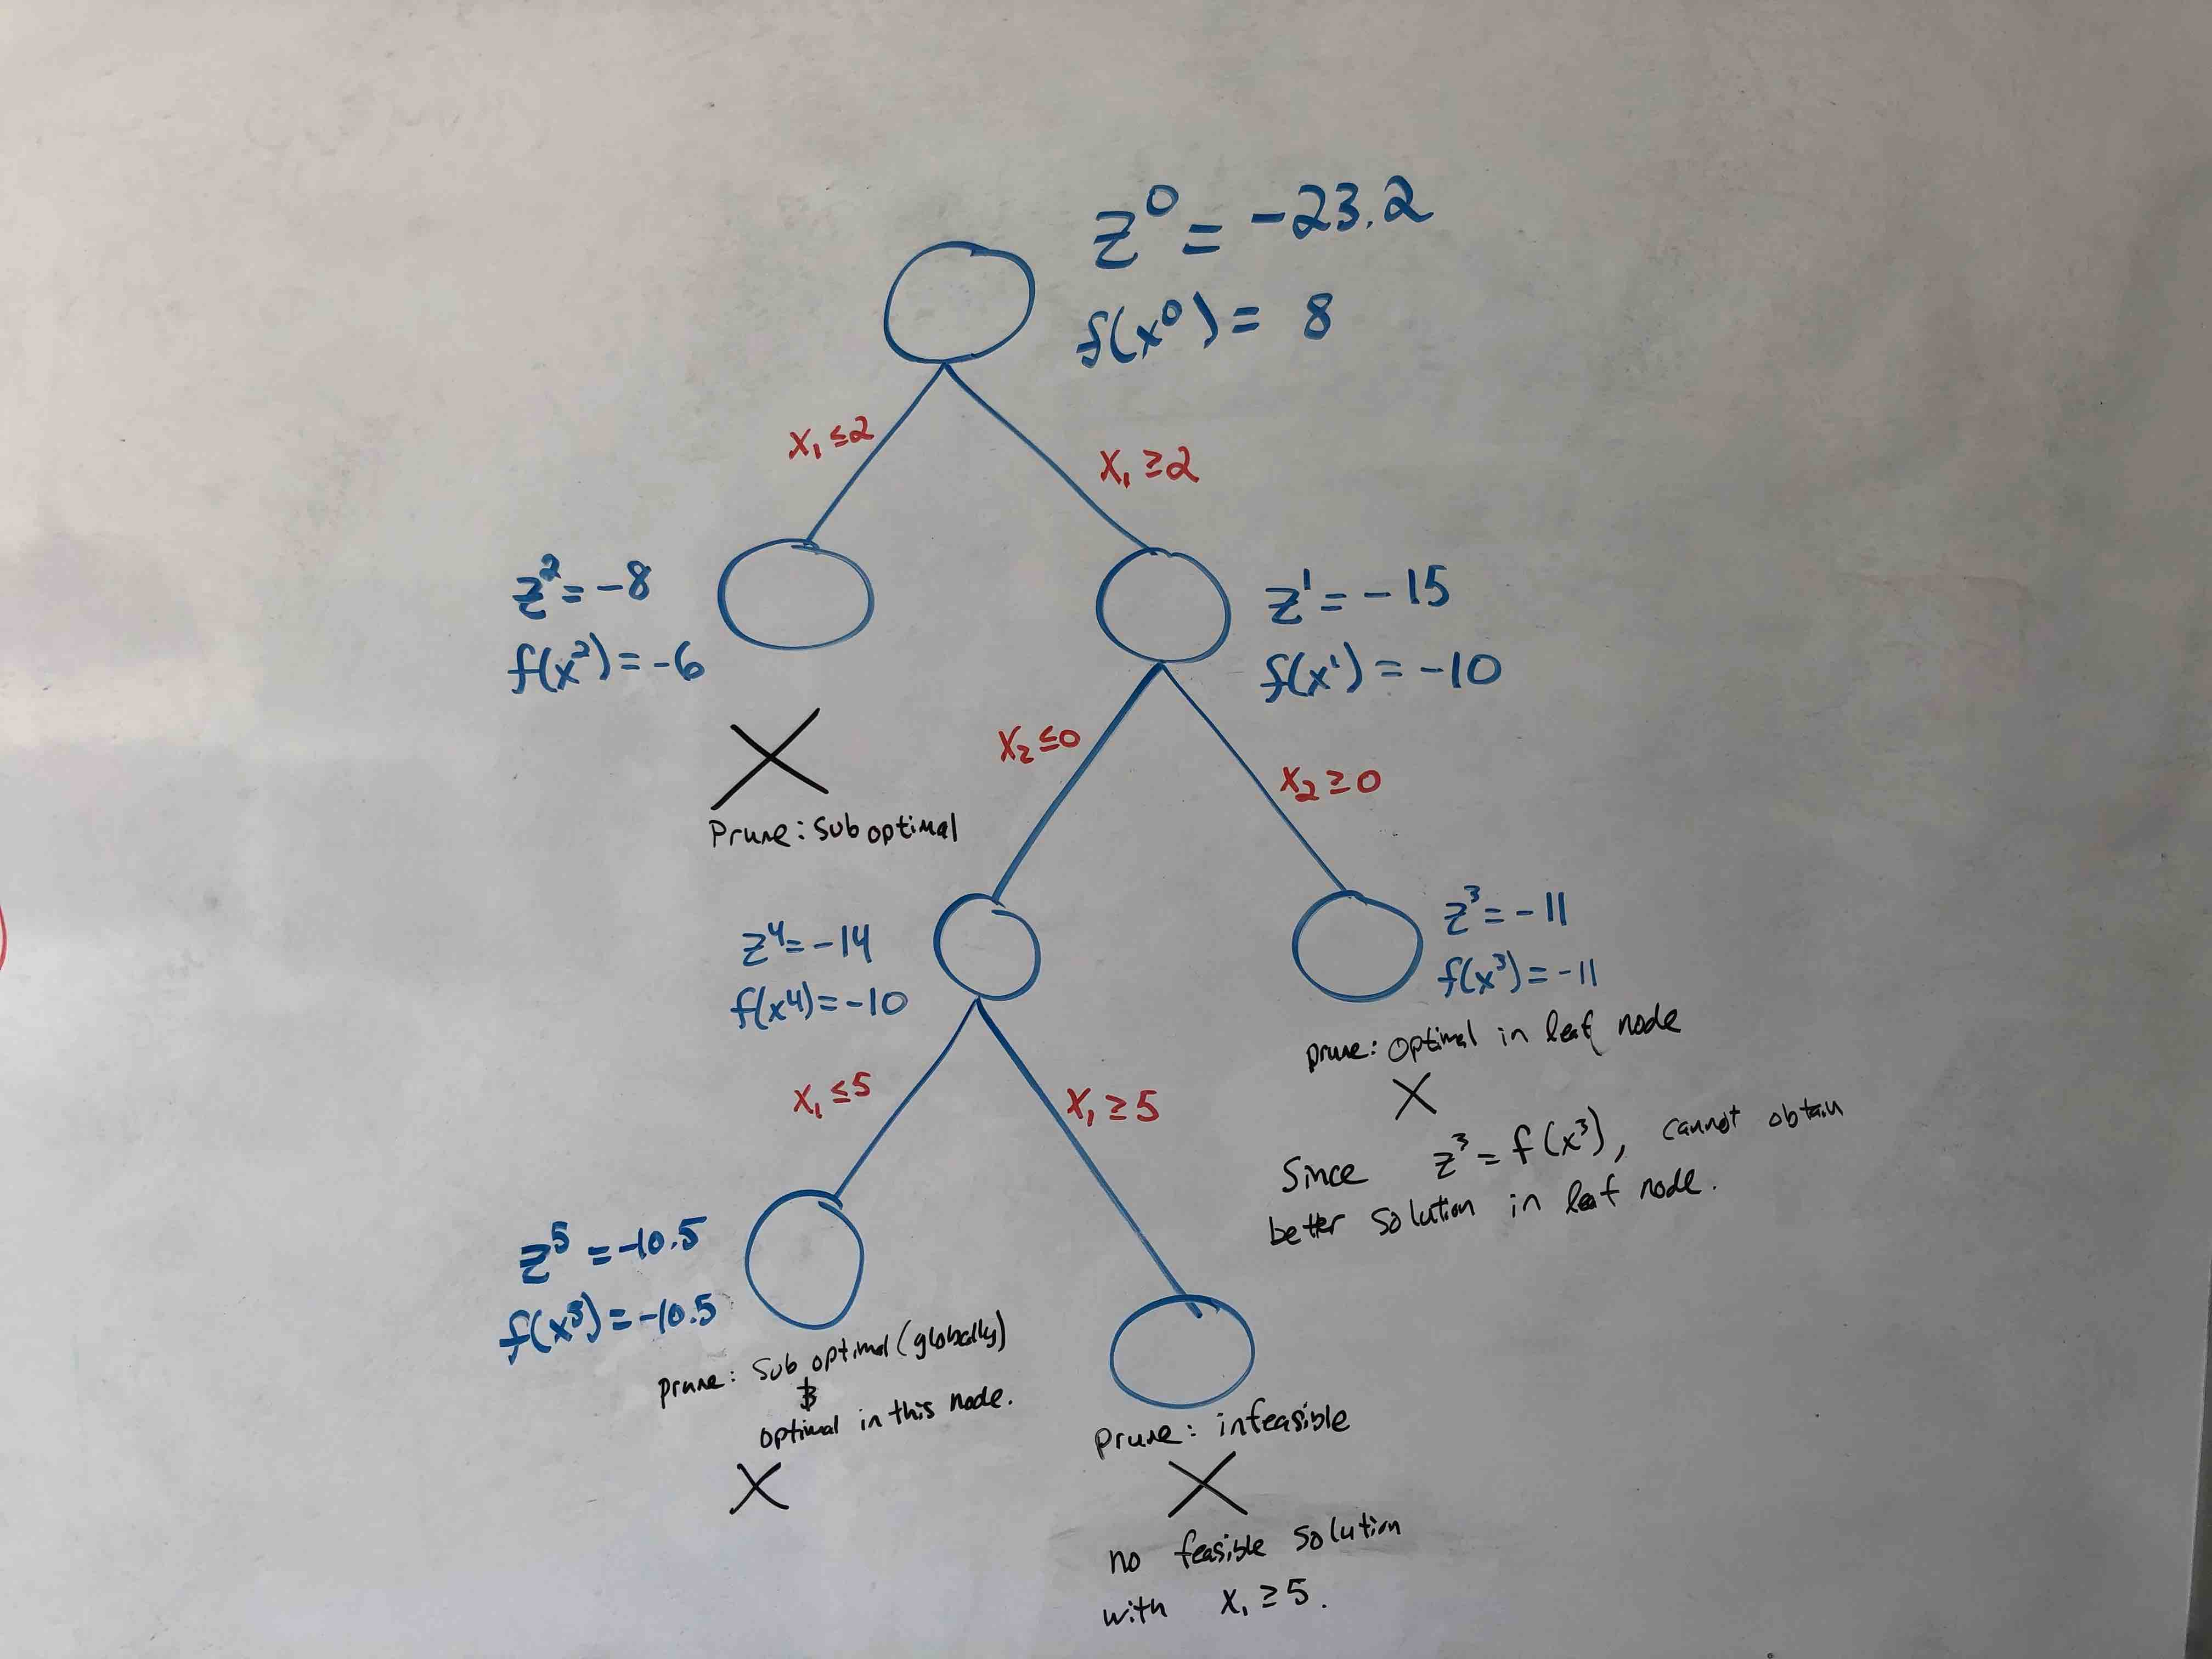
\includegraphics[scale = 0.1]{spatial_bnb_4}

Step 4:
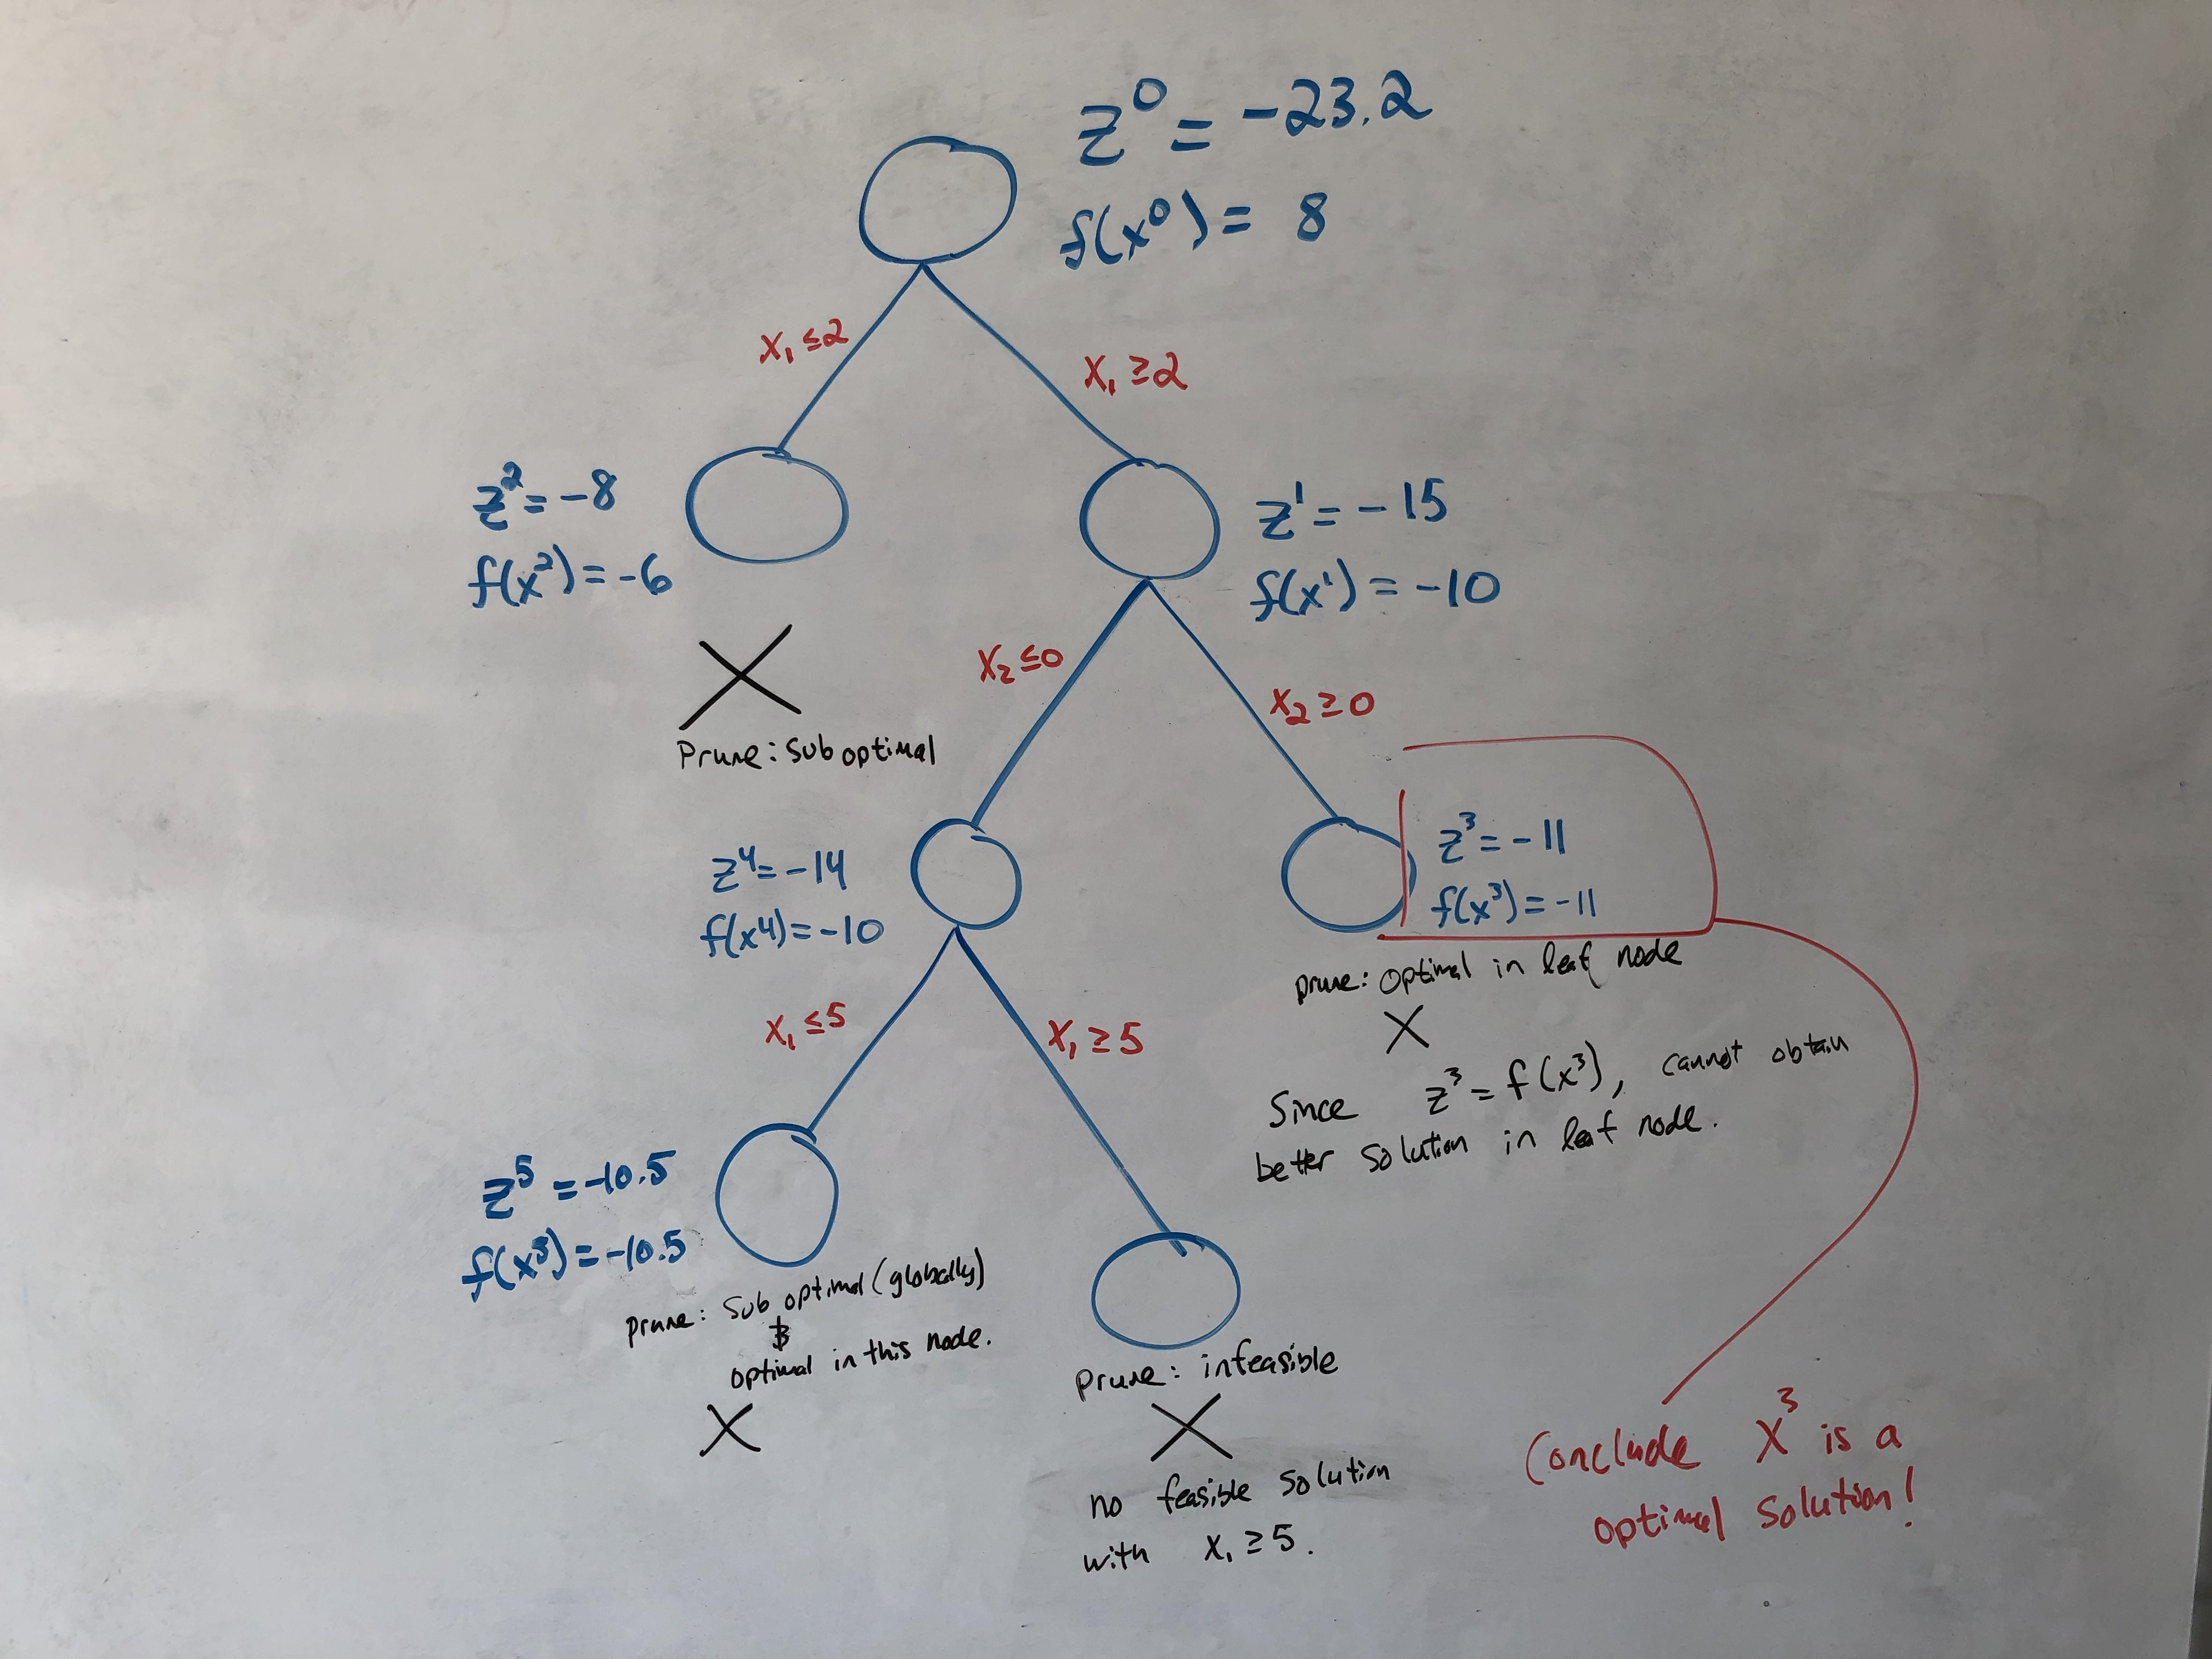
\includegraphics[scale = 0.1]{spatial_bnb_5}

\end{center}


There are several methods of construction relaxations $\R$ of $\F_\lift$ including McCormick envelopes, using more inequalities from the Boolean Quadric Polytope, or SDP relaxations.   These will be explored in the next few subsections.


\section{McCormick Envelope}
For two variables, $l_i \leq x_i \leq u_i$ and $l_j \leq x_j \leq u_j$, we first write these inequalties as 

\begin{align}
x_i - l_i \geq 0, \ \ \ u_i - x_i \geq 0\\
x_j - l_j \geq 0, \ \ \ u_j - x_j \geq 0
\end{align}

Multiplying any two inequalties yields a quadtaric inequality, that can be linearized using the $Y_{ij}$ variable.  For example, 

\begin{equation}
0 \leq (x_i - l_i) (x_j - l_j) = x_i x_j - l_i x_j - l_j x_i + l_i l_j = Y_{ij} - l_i x_j - l_j x_i + l_il_j.
\end{equation}

Enumerating all four pairs yields the McCormick Inequalities.

\begin{general}{McCormick Inequalities}{}
\begin{align}
 l_i x_j + l_j x_i - l_il_j \leq Y_{ij} \leq u_i x_j - l_j x_i + u_il_j\\
u_i x_j + u_j x_i - u_iu_j \leq Y_{ij} \leq  u_j x_i - l_i x_j + u_jl_i
\end{align}
\end{general}



\section{Relaxation Linearization Technique (RLT)}
The McCormic envelope inequalities are in fact a specific type of RLT inequality.  In particular, for any two valid inequalities
$$
a^1x \leq b_1
$$
$$
a^2x \leq b_2
$$
the inequality
$$
(a^1x - b_1)(a^2x - b_2) \geq 0
$$
is also a valid inequality.     
Using the lifted variables this could be rewritten as 
$$
\Gamma \circ Y + \beta^\top x + \alpha \geq 0
$$
which is a valid linear inequality for $\F_{\lift}$.  This inequality is referred to as an \emph{RLT inequality}.


\subsection{Boolean Quadric Polytope (BQP)}
In this section, we assume that the upper and lower bounds are normalized, that is, 
$$
0 \leq x \leq 1.
$$
This can be achieved easily by an affine transformation of the problem.  Alternatively, one can extract generalizations of the results in this section to arbitrary lower and upper bounds via an affine transformation in the reverse direction.

\begin{general}{Boolean Quadric Polytope (BQP)}{}
\begin{equation}
\BQP = \conv\left( (x,Y) \in \{0,1\}^{n+ E} | Y_{ij} = x_i x_j \ \ \forall (i,j) \in E \right)
\end{equation}
\end{general}

\begin{theorem}
\begin{equation}
\BQP = \conv\left( (x,Y) \in [0,1]^{n+ E} | Y_{ij} = x_i x_j \ \ \forall (i,j) \in E \right)
\end{equation}
\end{theorem}


\cite{Akshay-Gupte2019}
\begin{general}{Triangle Inequalities}{}
\begin{align*}
x_i + x_j + x_k - y_{ij} - y_{ik} - y_{jk} & \leq 1\\
- x_i + y_{ij} + y_{ik} - y_{jk} &\leq 0\\
- x_j + y_{ij} - y_{ik} + y_{jk}& \leq 0\\
- x_k - y_{ij} + y_{ik} + y_{jk} &\leq 0
\end{align*}
\end{general}

\begin{general}{Clique Inequalities}{}
$S \subseteq V$, $|S| \geq 3$, $1 \leq \alpha \leq |S|-2$, $\alpha \in \Z$
\begin{align*}
\alpha x(S) - y(E(S)) \leq \frac{\alpha(\alpha+1)}{2}
\end{align*}
\end{general}

\begin{general}{? Inequalities}{}

\end{general}

\subsection{SDP Relaxation}



\section{Lagrangian Relaxation}


Consider a polynomial optimization problem 

\section{New Results}

\begin{theorem}[Santana-Dey 2018]
Let $S = \{x \in \R^n : x^\top Q x + cT^\top x = g, x \in P\}$  for $P = \{x : Ax \leq b\}$ and $Q$ symmetric.  Then $\conv(S)$ is SOCr.  Proof is constructive.
\end{theorem}

\begin{theorem}[Gupte et. al. 2019]
If $G$ has nice structure, then $\BQP(G)$ has a polynomial size extended formulation.
\end{theorem}
\section{Polynomial Optimization - Algebraic Techniques}

\section{Cylindrical Algebraic Decomposition}


\section{Gr\"obner Bases}

\section{Quantifier Elimination and Semi-algebraic Sets}

\begin{theorem}
Any alternating quantifier set can be recast as a semi-algebraic set.
\end{theorem}




\chapter{Approximations of SOCP and SDP}
Some notes on applications for SDP: \url{http://www.seas.ucla.edu/~vandenbe/publications/sdp-apps.pdf}

\section{Outer linear approximation of SDP}
We describe a cutting plane technique for solving an SDP using Linear Programming and an oracle for finding eigenvectors of a matrix.   This cutting plane technique could be applied to many other types of problems.

\begin{general}{SDP}{}
\begin{align*}
\min  \quad & c^\top x\\
\text{ such that } \quad & Ax \leq b\\
& \sum_{i=1}^n F_i x_i + G \preceq 0 \tag{*} \label{eq:sdp-constraint}\\
&x \in \R^n
\end{align*}
\end{general}

Let $\xLP$ be the solution to the linear constraints to this problem, that is, we solve without the SDP constraint \eqref{eq:sdp-constraint}.  
\begin{itemize}
\item If $\xLP$ satisfies \eqref{eq:sdp-constraint}, then it is optimal.
\item Otherwise, we find a new inequality $d^\top x \leq f$ that is valid for the problem but cuts off $\xLP$.
\end{itemize}

Let $A  =  \sum_{i=1}^n F_i \xLP_i + G$.  If $A \not\preceq 0$, then we compute an eigenvector $v$ of $A$ with associated eigenvalue $\lambda > 0$.  

Then, 
\begin{equation}
v^\top \left( \sum_{i=1}^n F_i x_i + G\right)v \leq 0
\end{equation}
or equivalently
\begin{equation}
 \sum_{i=1}^nv^\top  F_iv x_i + v^\top Gv \leq 0
\end{equation}
is a valid inequality for the problem that cuts off $\xLP$.  Add this inequality to the LP and recompute $\xLP$.  Continue this process until $\xLP$ is feasible or close to feasible.

\chapter{Discretization Approaches}

\section{Complete discretization - all binary variables}
Let $x \in [l,u]$.  Then we can replace $x$ by an approximation in binary variables.  Most common is to replace
\begin{equation}
x = l +  \frac{1}{2^n} \sum_{i=1}^m 2^i \alpha_{i}
\end{equation}
where $m = \lceil log_2(u-l) \rceil$.  More generally, any integer base $b > 2$ can be used as 
\begin{equation}
x = l + \epsilon \sum_{i=1}^n b^i \left(\sum_{k=0}^b k \alpha_{ik}\right) \ \ \ \ \ \sum_{k=0}^b \alpha_{ik} = 1.
\end{equation}
Note that for $b=2$, we have variables $\alpha_{i0} + \alpha_{i1} = 1$, which reduces to the above case by eliminating the variable $\alpha_{i0}$.


Under this transformation, the main problem is now a binary problem.  Next, for any product appearing in the formilation,
$$
\prod_{i \in I} \alpha_i
$$
we can create a new variable $\beta_I = \prod_{i \in I} \alpha_i$.  Since $\alpha_i \in \{0,1\}$, $\beta_I \in \{0,1\}$, and we can model their equivalence as
\begin{equation}
\beta_I \leq \alpha_i  \ \ \text{ for all } i \in I \quad \text{ and } 1 + \sum_{i \in I} (\alpha_i-1) \leq \beta_I.
\end{equation}

Hence, the resulting formulation is a linear binary program in variables $\alpha_i$ and $\beta_I$.



\section{Products of continuous variables - NMDT}
We want to linearize the product of two variables using discretization.  That is, given 
\begin{equation}
\begin{split}
x =& s \cdot y\\
s_{\min} \leq &s \leq s_{\max}\\
y_{\min} \leq &y \leq y_{\max}
\end{split}
\end{equation}
we want to convert this to a linear model by using binary variables.  There are two main steps to this procedure.  First, we discretize $s$ into binary variables and then we model the product of each binary variable with the continuous variable $y$.
\subsection{Discretizing a continuous variable + small error}
\begin{general}{Discretizing a continuous variable + small error}{}
Suppose that we have a variable $z$ with bounds 
\begin{equation}
z_{\min} \leq z \leq z_{\max}.
\end{equation}
We can transform $z$ via a variable $w$ to the unit interval as 
\begin{equation}
\begin{split}
z &= (z_{\max} - z_{\min}) w + z_{\min}\\
0 \leq &w \leq 1
\end{split}
\end{equation}
Next, we can convert $w$ into a discrete variable $w_d\in \{ \tfrac{i}{2^n} : i=0,1,\dots, 2^n\}$ and an error $\Delta w \in [0, \tfrac{1}{2^n})$.  This gives us 
\begin{equation}
\begin{split}
z &= (z_{\max} - z_{\min}) (w_d + \Delta w) + z_{\min}\\
w_d&\in \{ \tfrac{i}{2^n} : i=0,1,\dots, 2^n\}\\
\Delta w &\in  [0,\tfrac{1}{2^n})
\end{split}
\end{equation}
Lastly, we convert the discrete $w_d$ into binary variables as $w_d = \sum_{i=1}^n 2^{-i} \alpha_i$ with $\alpha_i \in \{0,1\}$.  Thus we have 
\begin{equation}
\begin{split}
z &= (z_{\max} - z_{\min}) \left(\sum_{i=1}^n 2^{-i} \alpha_i + \Delta w\right) + z_{\min}\\
\alpha_i&\in \{0,1\}  \text{ for } i=1, \dots, n\\
\Delta w& \in [0,\tfrac{1}{2^n})
\end{split}
\end{equation}
\end{general}

\subsection{Binary and continuous variables}
\begin{general}{Modeling: product of binary and continuous variable}{}
\begin{equation}
\begin{split}
x &= \delta \cdot y\\
y_{\min} \leq &y \leq y_{\max}\\
\delta &\in \{0,1\}
\end{split}
\end{equation}
\end{general}

Thus, we want to have the following happen
\begin{equation}
x = \begin{cases}
y & \text{ if } \delta = 1\\
0 & \text{ if } \delta = 0
\end{cases}
\end{equation}


This can be accomplished by 
\begin{general}{Modeling: product of binary and continuous variable - Reformulation}{}
\begin{equation}
\begin{split}
\delta y_{\min} \leq &x \leq \delta y_{\max}\\
(1-\delta) y_{\min} \leq &\bar x \leq (1-\delta) y_{\max}\\
y &=  x + \bar x\\
\delta& \in \{0,1\}
\end{split}
\end{equation}
\end{general}
Alternatively, we can eliminate the variable $\bar x$ by $\bar x = y - x$, leaving us with
\begin{general}{Modeling: product of binary and continuous variable - Equivalent reformulation}{}
\begin{equation}
\begin{array}{rrcll}
\delta y_{\min} &\leq &x &\leq \delta y_{\max}\\
%y - (1-\delta) y_{\max} \leq &x \leq y - (1-\delta) y_{\min}\\
(1-\delta) y_{\min} &\leq &y-x &\leq   (1-\delta) y_{\max}\\
 & & \delta &\in \{0,1\}
\end{array}
\end{equation}
\end{general}

\subsection{References}
\cite{doi:10.1080/10556788.2016.1264397}

